\frame{
\frametitle{\secname}

\begin{columns}
\column{0.6\textwidth}
\begin{itemize}
\item Clocks wrap around after 24h\footnote{Ignoring the fact that DST just ended}
\item Generalize by fixing a \emph{modulus} $m$, and do all math as remainders when dividing by $m$
\begin{itemize}
\item All integers $x=qm+r$ are treated as the same number
\end{itemize}
\item When to compute remainders?
\begin{itemize}
\item $(q_1m+r_1)+(q_2m+r_2)=(q_1+q_2)m+r_1+r_2$.
\item $(q_1m+r_1)\cdot(q_2m+r_2)=(q_1q_2m+q_1r_2+r_1q_2)m+r_1r_2$.
\end{itemize}
\end{itemize}

\column{0.4\textwidth}
\begin{figure}
\centering
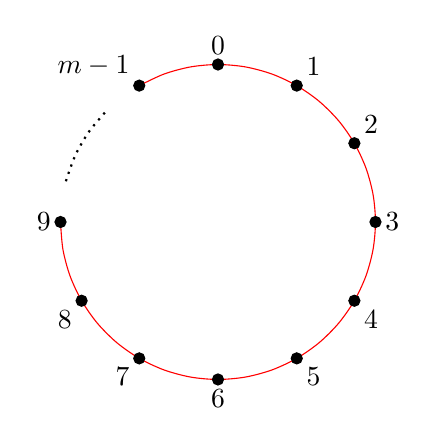
\begin{tikzpicture}
\def\r{2}
\draw[color=red,smooth,every node/.style={color=black},mark=*,mark size=2pt,mark options={color=black}]
    plot[domain=-30:270,samples=31,mark repeat=3] ({\r*cos(90-\x)},{\r*sin(90-\x)});
\draw[dotted,thick,smooth,every node/.style={color=black},mark=]
    plot[domain=285:315,samples=4] ({\r*cos(90-\x)},{\r*sin(90-\x)});
\node[above] (0) at (90:\r) {0};
\node[above right] (1) at (60:\r) {1};
\node[above right] (2) at (30:\r) {2};
\node[right] (2) at (0:\r) {3};
\node[below right] (2) at (-30:\r) {4};
\node[below right] (2) at (-60:\r) {5};
\node[below] (2) at (-90:\r) {6};
\node[below left] (2) at (-120:\r) {7};
\node[below left] (2) at (-150:\r) {8};
\node[left] (2) at (-180:\r) {9};
\node[above left] (3) at (120:\r) {$m-1$};
\end{tikzpicture}
\end{figure}


\end{columns}

}